% --- NASTAVENÍ DOKUMENTU ---
\documentclass[10pt, a4paper]{report}

\usepackage[utf8]{inputenc}
\usepackage[czech]{babel}
\usepackage{csquotes}
\usepackage[T1]{fontenc}
\usepackage{lmodern}

\usepackage{float}
\usepackage{caption}
\usepackage{nameref}
\usepackage{amsmath}
\usepackage{graphicx}
\usepackage[hidelinks]{hyperref}
\usepackage{titlesec}
\usepackage{todonotes}
\usepackage[
left=30mm,
right=30mm,
top=40mm,
bottom=30mm,
]{geometry}

% --- DOKUMENTACE ---
\begin{document}
	
	% Titulek
	\pagenumbering{arabic}
	\thispagestyle{empty}
	
	\begin{titlepage}
		\centering
		
		{\Large Úvod do paralelního programování} \\[0.5cm]
		{\Large 1. Semestrální práce} \\[2.5cm]
		
		{\huge \bfseries Analýza meteorologických dat} \\[0cm]
		
		\vfill
		
		\begin{flushleft} \small
			Jméno: Jan Kopačka \\
			Osobní číslo: A24B0346P \\
			Email: jankop@students.zcu.cz \\
			Datum: \today
		\end{flushleft}
		
	\end{titlepage}
	
	% Obsah
	\setcounter{page}{2}
	
	\tableofcontents
	\newpage
	
	\chapter{Úvod}
	
	Cílem této semestrální práce je návrh a implementace vysoce výkonné aplikace pro analýzu a vizualizaci meteorologických dat z území České republiky. Práce vychází z reálných měření poskytnutých Českým hydrometeorologickým ústavem (ČHMÚ), která byla pro účely testování škálovatelnosti rozšířena do tří úrovní obtížnosti (malá, střední a velká datová sada).
	
	Hlavním úkolem aplikace je zpracování dvou typů vstupních dat v textovém formátu CSV: seznamu měřicích stanic a souboru obsahujícího průměrné denní teploty. Zpracování zahrnuje několik klíčových fází:
	\begin{itemize}
		\item \textbf{Předzpracování a filtrace:} Identifikace stanic s dostatečnou kvalitou dat, definovanou jako přítomnost alespoň 5 let souvislých měření a průměrná hustota záznamů vyšší než 100 hodnot ročně.
		\item \textbf{Detekce anomálií:} Vyhledávání meziročních výkyvů teplot v jednotlivých měsících na základě statistického prahu (75 \% celkového rozpětí teplot dané stanice v daném měsíci).
		\item \textbf{Vizualizace:} Generování dvanácti map České republiky ve formátu SVG (jedna pro každý kalendářní měsíc), kde jsou stanice barevně interpolovány na škále modrá–žlutá–červená podle průměrných teplot.
	\end{itemize}
	
	Z technického hlediska je kladen důraz na efektivitu a paralelizaci výpočtů. Aplikace je implementována v jazyce C++ s využitím knihovny \textbf{OpenMP} pro distribuci zátěže mezi více jader procesoru. Program umožňuje běh v sériovém i paralelním režimu, což slouží k následné analýze výkonu, výpočtu reálného urychlení a ověření teoretických předpokladů na základě Amdahlova a Gustafsonova zákona.
	
	Dokumentace v následujících kapitolách podrobně popisuje zvolenou architekturu, proces identifikace úseků vhodných pro paralelizaci a vyhodnocení naměřených výsledků na testovacím hardwaru.
	
	\chapter{Vývojové a testovací prostředí}
	\section{Softwarové prostředí}
	Program byl vyvíjen na operačním systému Windows 11 Pro. Jako hlavní vývojové prostředí (IDE) bylo využito CLion od společnosti JetBrains, přičemž o překlad se staral kompilátor g++ v prostředí MinGW. Pro ověření kompatibility a správného fungování byl kód rovněž odzkoušen v prostředí Microsoft Visual Studio 2022 s využitím překladače MSVC.
	
	\section{Hardwarové vybavení}
	Vývoj aplikace a měření prezentovaných výsledků probíhalo na počítačové sestavě s následující specifikací:
	\begin{itemize}
		\item \textbf{Procesor (CPU):} AMD Ryzen 5 7600X (6 fyzických jader, 12 vláken)
		\item \textbf{Operační paměť (RAM):} 32 GB DDR5 (6000 MHz, CL36)
		\item \textbf{Grafická karta (GPU):} NVIDIA GeForce RTX 4070 (12 GB GDDR6X)
		\item \textbf{Úložiště:} 1 TB NVMe SSD (Kingston KC3000)
	\end{itemize}
	
	\chapter{Analýza úlohy a implementace}
	\section{Rozdělení modulů}
	Pro dosažení čistoty kódu byly jednotlivé úlohy seskupeny do několika modulů podle jejich charakteru. Seznam úloh je vizuálně popsán v kapitole Precedenční graf.
	
	\subsection{Modul vstupu (data\_loader.h, data\_loader.cpp)}
	Tento modul zapouzdřuje tasky, které pracují s externími zdroji dat a transformují je do vnitřních struktur aplikace.
	\begin{itemize}
		\item \textbf{Načtení stanic} – Prvotní inicializace mapy stanic ze souboru \texttt{stanice.csv}.
		\item \textbf{Načtení measurements} – Naplnění existujících struktur daty ze souboru \texttt{mereni.csv}.
	\end{itemize}
	
	\subsection{Modul zpracování (data\_processor.h, data\_processor.cpp)}
	Zde probíhá výpočetně nejnáročnější zpracování dat. Modul obsahuje úlohy, které mění stav datové sady nebo z ní extrahují nové informace.
	\begin{itemize}
		\item \textbf{Filtrace stanic} – Odstranění stanic nesplňujících podmínku 5 let souvislých dat a průměrného počtu měření. Součástí je i předvýpočet statistik.
		\item \textbf{Detekce anomálií} – Algoritmus pro identifikaci meziročních teplotních výkyvů na základě 75\% prahu.
	\end{itemize}
	
	\subsection{Modul výstupu (output\_generator.h, output\_generator.cpp, czmap\_svg.h)}
	Tento modul se stará o tasky spojené s prezentací výsledků.
	\begin{itemize}
		\item \textbf{Export anomálií} – Zápis nalezených výkyvů do souboru \texttt{vykyvy.csv}.
		\item \textbf{Export SVG} – Generování 12 map s lineární interpolací souřadnic a barevnou škálou.
	\end{itemize}
	
	\subsection{Společná infrastruktura (data\_types.h, main.cpp)}
	\begin{itemize}
		\item \textbf{data\_types.h}: Obsahuje definice struktur \texttt{Station}, \texttt{Measurement} a \texttt{Anomaly}. Tyto struktury představují pevně definované datové rozhraní mezi všemi moduly.
		\item \textbf{main.cpp}: Funguje jako hlavní řídicí bod, který tasky spouští v pořadí definovaném v precedenčním grafu.
	\end{itemize}
	
	\section{Paralelizace}
	\subsection{Precedenční graf}
	Časy v precedenčním grafu a tabulce jsou ze sériové varianty na velkých datech. Hodnoty jsou skutečně naměřené, avšak v tomto kontextu slouží spíše jako referenční ukázka a kontext k precedenčnímu grafu.
	
	\begin{figure}[H]
		\centering
		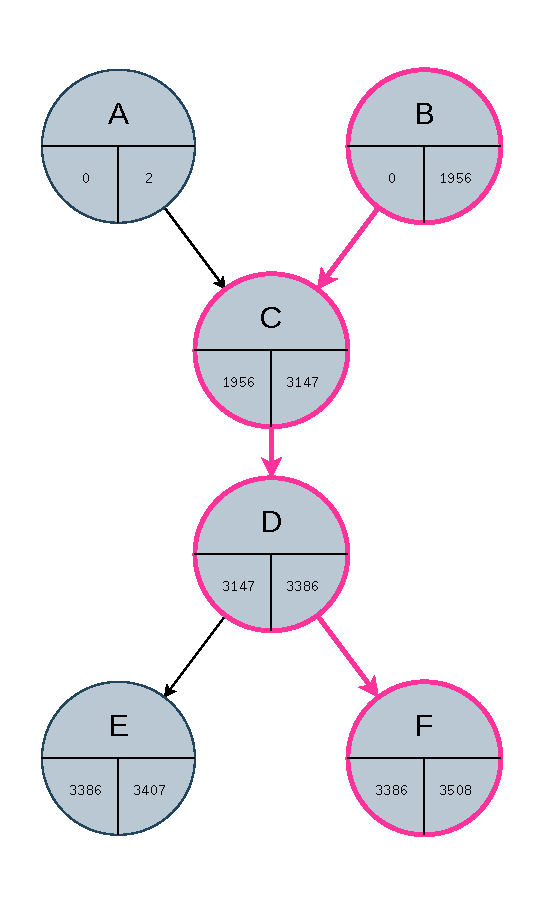
\includegraphics[width=0.5\textwidth]{graph.pdf}
		\caption{Precedenční graf se znázorněnou kritickou cestou}
		\label{fig:graph}
	\end{figure}
	
	\begin{table}[H]
		\centering
		\begin{tabular}{|c|l|c|}
			\hline
			\textbf{Označení} & \textbf{Popis} & \textbf{Pr. čas (ms)} \\ \hline
			A & Načtení stanic z CSV souboru & 2 \\ \hline
			B & Načtení měření jednotlivých stanic z CSV souboru & 1956 \\ \hline
			C & Filtrace stanic na základě jejich měření & 1191 \\ \hline
			D & Detekce anomálií stanic, které byly zachovány & 239 \\ \hline
			E & Export CSV souboru anomálií & 21 \\ \hline
			F & Export 12 SVG map pro každý měsíc & 122 \\ \hline
		\end{tabular}
		\caption{Precedenční graf: úlohy a naměřené časy}
	\end{table}
	
	\subsection{Kritická cesta a průměrná míra paralelismu} \label{sec:kriticka_cesta}
	Nejprve stanovíme celkový objem práce $T$ (Total Work), který odpovídá součtu časů všech podúloh v sériovém režimu:
	\begin{equation}
		T = A + B + C + D + E + F = 2 + 1956 + 1191 + 239 + 21 + 122 = 3531 \text{ ms}
	\end{equation}
	
	Dále identifikujeme délku kritické cesty $L$ (Critical Path), představující nejdelší možnou posloupnost na sobě závislých úloh. V našem případě vede tato cesta přes uzly $B \to C \to D \to F$:
	\begin{equation}
		L = 1956 + 1191 + 239 + 122 = 3508 \text{ ms}
	\end{equation}
	
	Z těchto hodnot lze vypočítat průměrnou míru paralelismu $d$, která udává teoretické urychlení v případě paralelizace výhradně na úrovni úloh (Task Parallelism):
	\begin{equation}
		d = \frac{T}{L} = \frac{3531}{3508} \approx 1,007 \text{}
	\end{equation}
	Tato hodnota blízká 1 potvrzuje, že závislosti mezi úlohami jsou natolik silné, že souběžné spouštění celých tasků (např. pomocí \texttt{omp sections}) nepřináší významný výkonnostní zisk.
	
	\subsection{Identifikace vhodných míst pro paralelizaci}
	Největší zrychlení bylo potřeba v načítání souborů. Zde se uplatnil fakt, že ačkoliv nelze paralelizovat čisté čtení z disku, následný převod do vnitřních struktur paralelizovat lze.
	
	Na základě analýzy výpočetní složitosti a datových závislostí byly identifikovány následující úseky vhodné pro uplatnění paralelismu:
	
	\subsubsection*{Fáze načítání a parsování dat}
	Zpracování textových vstupů je rozděleno na sekvenční čtení do paměťového bufferu a následné paralelní parsování. Buffer je rozdělen na bloky (chunks), jejichž hranice jsou dynamicky zarovnány na znak konce řádku, aby nedošlo k poškození záznamů. Každé vlákno pracuje s vlastní lokální strukturou, čímž se minimalizuje potřeba synchronizace; ke sloučení dat dochází až v kritické sekci po dokončení parsování daného bloku.
	
	\subsubsection*{Fáze filtrace stanic}
	Filtrace probíhá iterací přes vektor stanic, kde se pro každou stanici nezávisle ověřují podmínky na délku souvislého měření a frekvenci dat. Aby se předešlo neefektivní manipulaci s pamětí při paralelním odstraňování prvků, je využita pomocná maska (vektor příznaků), do které vlákna zapisují výsledky validace bez nutnosti vzájemné synchronizace. Samotné sestavení výsledného vektoru je pak provedeno sekvenčně, což eliminuje režii spojenou s paralelní alokací.
	
	\subsubsection*{Fáze detekce anomálií}
	Algoritmus detekce anomálií vyhodnocuje meziroční teplotní výkyvy pro každou stanici izolovaně. Vlákna v paralelním cyklu nezávisle vypočítávají lokální prahové hodnoty a identifikují skoky v datech. Vzhledem k nízké pravděpodobnosti výskytu anomálie v poměru k celkovému objemu dat je pro vkládání výsledků do sdíleného vektoru použita kritická sekce, jejíž režie je v tomto případě zanedbatelná.
	
	\subsubsection*{Fáze generování výstupů}
	Při generování vizualizací je nejprve využita paralelní redukce pro zjištění globálního teplotního minima a maxima napříč všemi měřeními, což je nezbytné pro kalibraci barevné škály. Samotný export 12 SVG map je paralelizován na úrovni jednotlivých měsíců. Každé vlákno obsluhuje vlastní souborový proud, což umožňuje paralelní zápis na disk bez nutnosti synchronizace přístupu k souborům. Export do hlavního CSV souboru byl ponechán jako sekvenční operace, aby se předešlo vysoké režii spojené s koordinací zápisu do jednoho sdíleného souboru.
	
	\section{Implementace}
	
	\subsection{Stručný popis}
	
	Pro paralelizaci výpočtů byla zvolena knihovna \textbf{OpenMP}. Hlavním důvodem této volby je zachování vysoké přehlednosti a čistoty zdrojového kódu. Paralelizace je realizována pomocí direktiv kompilátoru (\texttt{\#pragma omp}), které umožňují transformovat kritické úseky algoritmu na paralelní bez nutnosti rozsáhlého refaktoringu nebo implementace komplexní správy vláken. Tento přístup zajišťuje, že kód zůstává srozumitelný a blízký své sekvenční logice.
	
	Program disponuje mechanismem pro přepínání mezi sekvenčním a paralelním vykonáváním na bázi příznaku \textbf{\texttt{is\_parallel}}. Tento logický parametr je inicializován v modulu \texttt{main.cpp} analýzou argumentů příkazové řádky (\texttt{---serial} nebo \texttt{---parallel}). Hodnota příznaku je následně distribuována do všech klíčových metod loaderu, procesoru i generátoru. Většina paralelních bloků v kódu využívá podmíněnou klauzuli \texttt{if(is\_parallel)}, což zaručuje identické chování algoritmu v obou režimech a eliminuje režii OpenMP v případech, kdy je vyžadován sériový běh.
	
	\textbf{Tok dat} mezi jednotlivými moduly je navržen pro maximální efektivitu a nízkou paměťovou režii:
	\begin{enumerate}
		\item \textbf{Načítání (Modul vstupu):} Data jsou parsována z CSV souborů. Pro úvodní přiřazení měření ke stanicím je využita \texttt{std::unordered\_map} pro dosažení konstantní časové složitosti vyhledávání podle ID stanice.
		\item \textbf{Transformace:} Jakmile jsou všechna data v paměti, hash mapa je převedena na \texttt{std::vector}. Tento krok je klíčový pro následnou paralelizaci, protože souvislé uložení v paměti umožňuje optimální využití CPU cache a snadné rozdělení iteračního prostoru mezi vlákna.
		\item \textbf{Zpracování (Modul zpracování):} Nad vektorem stanic probíhá filtrace (odstranění stanic nesplňujících kritéria) a výpočetní analýza pro detekci anomálií. Výsledkem je vektor struktur \texttt{Anomaly}.
		\item \textbf{Výstup (Modul výstupu):} Data o anomáliích jsou sekvenčně zapsána do CSV souboru. Současně probíhá paralelní generování 12 SVG map, kde každé vlákno nezávisle konstruuje grafickou reprezentaci pro konkrétní měsíc v roce.
	\end{enumerate}
	
	\subsection{Další učiněná rozhodnutí a vysvětlení implementačních detailů}
	
	\subsubsection{Filtrace stanic}
	
	Hlavním cílem této sekce je upřesnit způsob filtrování stanic. Důvodem je to, že v zadání je v rámci této části drobný prostor pro vlastní interpretaci. 
	
	Základním kritériem je počet let, přičemž pokud má stanice záznamy z méně než 5 různých let, je z dalšího zpracování vyřazena. Toto je nejrychlejší filtr.
	
	Důležitá je také souvislost let. Pokud stanice měřila například v letech 1990–1993 (4 roky) a pak až v letech 2000–2003 (další 4 roky), má sice 8 let dat, ale neprojde, protože její nejdelší souvislý blok je pouze 4 roky dlouhý. Pro úspěšnou filtraci musí existovat alespoň jeden blok o délce minimálně 5 let.
	
	Dalším požadavkem je dostatečná frekvence měření. Pokud stanice měřila například v období let 2000 až 2010 (období 11 let), musí mít v součtu alespoň 1100 záznamů, aby byla považována za dostatečně aktivní. Toto pravidlo platí i v případě, kdy stanice měřila pouze v roce 2000 a posléze až v roce 2010. Situace se interpretuje jako období od 2000 do 2010 (11 let), a ačkoliv reálně probíhalo měření jen dva roky, výpočet požadované frekvence je identický a je třeba dosáhnout 1100 záznamů.
	
	\subsubsection{Práce s I/O operacemi}
	
	Vstupní soubory jsou otevírány v binárním režimu pomocí příznaku \texttt{std::ios::binary}. Tento krok primárně zrychluje proces čtení, jelikož operační systém nemusí provádět skrytou textovou konverzi konců řádků (např. \texttt{\textbackslash r\textbackslash n} na \texttt{\textbackslash n} ve Windows). Dává nám to absolutní kontrolu nad parsováním formátu a správným rozdělením znaků, přičemž celý soubor je načten naráz do alokovaného paměťového bufferu, abychom minimalizovali I/O operace.
	
	Paralelizace čtení je umožněna tím, že je soubor načten do jednoho velkého řetězce, který program následně rozdělí na bloky (chunks) odpovídající počtu dostupných vláken. Hranice každého bloku se dynamicky posunou na nejbližší znak konce řádku (\texttt{\textbackslash n}), aby se předešlo přeseknutí záznamu v polovině. Každé vlákno pak nezávisle parsuje pouze svůj vymezený paměťový blok.
	
	Samotný zápis výsledných anomálií do CSV souboru (\texttt{export\_anomalies}) byl ponechán jako sekvenční operace. Snaha o paralelizaci zápisu do jednoho sdíleného souboru by vyžadovala striktní synchronizaci pomocí kritických sekcí nebo zámků, jejíž režie by při předpokládaném objemu výsledků zcela eliminovala jakékoliv zrychlení. Paralelní tak zůstává pouze výpočet a formátování obsahu pro nezávislé SVG soubory.
	
	Pro dosažení maximální propustnosti dat probíhá parsování číselných hodnot z bufferu zcela manuálně pomocí přímé manipulace s ASCII znaky (např. výpočtem \texttt{id = id * 10 + (buffer[pos] - '0')}), čímž se zcela vyhýbáme volání standardních funkcí jako \texttt{std::stoi} nebo \texttt{std::atof}. Tento přístup eliminuje režii spojenou s alokací pomocných řetězců, kontrolou lokalizace a vnitřní stavovou logikou standardních proudů, která je při zpracování milionů řádků kritickým úzkým hrdlem. V kombinaci s předem načteným bufferem tato nízkoúrovňová optimalizace umožňuje dosáhnout řádově vyššího výkonu, což je pro efektivní využití paralelních vláken u datově intenzivních úloh klíčové.
	
	\subsubsection{Volba datových struktur}
	
	Při volbě datových struktur je pro počáteční načtení měření využita \texttt{std::unordered\_map} (hash mapa). Hlavním důvodem je nutnost okamžitého vyhledávání stanice dle jejího ID pro přiřazení naměřené hodnoty se složitostí $O(1)$. V polovině procesu, těsně před započetím analytických výpočtů, je však obsah hash mapy přesunut do souvislého paměťového bloku \texttt{std::vector}. Vektory lépe využívají paměť typu CPU cache a především umožňují efektivní a korektní rozdělení práce v blocích při použití \texttt{\#pragma omp parallel for}.
	
	Aby byla zajištěna férovost měření, probíhá tento paměťový převod zcela shodně jak v paralelní, tak v sériové variantě běhu programu. Smyslem je zajistit maximální jednotnost algoritmické logiky a paměťové stopy. Pouze v případě, že sériová verze provádí identickou režii, jsou získané metriky zrychlení spravedlivé a skutečně vypovídají o čistém výkonnostním zisku ze zapojení více vláken do výpočtů.
	
	\subsubsection{Specifika využití knihovny OpenMP}
	
	Z hlediska datových typů iterátorů mohl být díky využití standardu OpenMP 3.0+ použit pro iterační proměnné v paralelních for cyklech typ \texttt{size\_t} namísto tradičních znaménkových celých čísel (\texttt{int}). Při iteraci přes rozsáhlé kolekce dat, jakou je například \texttt{std::vector}, představuje \texttt{size\_t} nativní a mnohem bezpečnější řešení, jež zamezuje potenciálnímu přetečení u extrémně velkých souborů.
	
	Specifickým rozhodnutím bylo vyloučení vnořeného paralelismu a sekcí (omp sections). Precedenční graf by teoreticky nabízel možnost spouštět některé odlišné tasky paralelně vedle sebe, například načítat stanice a měření ve stejný čas, nicméně tato metoda nebyla implementována. Knihovna OpenMP je totiž navržena tak, že každá úroveň paralelizace alokuje všechna smysluplná vlákna (např. 12 vláken pro CPU). Kdyby došlo ke spuštění více tasků paralelně nad sebou, systém by masivně překročil počet hardwarových vláken (oversubscription). Místo zrychlení by došlo k extrémnímu nárůstu režie na přepínání kontextů operačního systému a výkon by se naopak propadl. Z tohoto důvodu program paralelizuje data výhradně na úrovni dat uvnitř jednotlivých tasků.
	
	Toto tvrzení bylo navíc potvrzeno v sekci \ref{sec:kriticka_cesta}, kde průměrná míra paralelismu vyšla velmi blízko hodnotě 1. To je jednoznačný ukazatel, že úlohy jsou na sobě silně závislé a pralelizace na úrovni úloh, by mohlo být kvůli vyšší režii spíše na škodu.
	
	\subsubsection{Zjednodušení distribuce šablony}
	Aby se minimalizovala chybovost a složitost nasazení aplikace u koncového uživatele (například špatně zadaná relativní cesta z příkazové řádky), byl vizuální základ slepé mapy (\texttt{<?xml version="1.0" ... <svg>}) vložen přímo do hlavičkového souboru \texttt{czmap\_svg.h} jako takzvaný surový řetězec (raw string literal \texttt{R"(...)"}). Aplikace tak nepotřebuje žádné externí zdrojové soubory a vystačí si (teoreticky) čistě se zkompilovanou binárkou.
	
	\subsection{Naměřené hodnoty}
	
	\begin{table}[h]
		\centering
		\renewcommand{\arraystretch}{1.2}
		\begin{tabular}{|l|c|c|}
			\hline
			\textbf{Datová sada} & \textbf{Sériová verze [ms]} & \textbf{Paralelní verze [ms]} \\ \hline
			Malá & 154 & 82 \\ \hline
			Střední & 1 850 & 412 \\ \hline
			Velká & 3 531 & 325 \\ \hline
		\end{tabular}
		\caption{Naměřené časy zpracování pro různé velikosti datových sad.}
		\label{tab:mereni_vykonu}
	\end{table}
	
	\chapter{Metriky relativní k paralelizaci}
	
	\section{Urychlení}
	
	Následující část se věnuje vyhodnocení efektivity paralelizace výhradně na velké datové sadě, kde se naplno projevuje vliv distribuce zátěže mezi jednotlivá jádra procesoru. V tabulce jsou uvedeny časy pro jednotlivé úlohy (tasky) definované v precedenčním grafu.
	
	\begin{table}[h]
		\centering
		\renewcommand{\arraystretch}{1.2}
		\begin{tabular}{|l|c|c|}
			\hline
			\textbf{Úloha (Task)} & \textbf{Sériová varianta [ms]} & \textbf{Paralelní varianta [ms]} \\ \hline
			Načtení stanic (A) & 2 & 2 \\ \hline
			Načtení měření (B) & 1956 & 923 \\ \hline
			Filtrace stanic (C) & 1191 & 201 \\ \hline
			Detekce anomálií (D) & 239 & 23 \\ \hline
			Export anomálií (E) & 21 & 20 \\ \hline
			Export SVG map (F) & 122 & 210 \\ \hline
			Ostatní & 39 & 71 \\ \hline
			\hline
			\textbf{Celkový čas} & \textbf{3570} & \textbf{1379} \\ \hline
		\end{tabular}
		\caption{Srovnání časů jednotlivých úloh na velké datové sadě.}
		\label{tab:velka_data_detaily}
	\end{table}
	
	Na základě celkových naměřených časů lze vypočítat reálné urychlení $S$ (speedup) aplikace podle následujícího vztahu:
	
	\begin{equation}
		S = \frac{T_{\text{sériová}}}{T_{\text{paralelní}}} = \frac{3597}{1379} \approx 2,59
	\end{equation}
	
	Dosažené reálné urychlení $S \approx 2,59$ na 12vláknovém procesoru ukazuje na výrazné zrychlení výpočetně náročných částí (B, C, D). Výsledek potvrzuje, že pro rozsáhlé meteorologické soubory je paralelní zpracování kritické pro dosažení akceptovatelné odezvy systému.
	
	\chapter{Metriky relativní k paralelizaci}
	
	\section{Urychlení}
	
	Následující část se věnuje vyhodnocení efektivity paralelizace výhradně na velké datové sadě, kde se naplno projevuje vliv distribuce zátěže mezi jednotlivá jádra procesoru. V tabulce jsou uvedeny časy pro jednotlivé úlohy (tasky) definované v precedenčním grafu.
	
	\begin{table}[H]
		\centering
		\renewcommand{\arraystretch}{1.2}
		\begin{tabular}{|l|c|c|}
			\hline
			\textbf{Úloha (Task)} & \textbf{Sériová varianta [ms]} & \textbf{Paralelní varianta [ms]} \\ \hline
			Načtení stanic (A) & 2 & 2 \\ \hline
			Načtení měření (B) & 1956 & 923 \\ \hline
			Filtrace stanic (C) & 1191 & 201 \\ \hline
			Detekce anomálií (D) & 239 & 23 \\ \hline
			Export anomálií (E) & 21 & 20 \\ \hline
			Export SVG map (F) & 122 & 210 \\ \hline
			Ostatní & 39 & 71 \\ \hline
			\hline
			\textbf{Celkový čas} & \textbf{3570} & \textbf{1450} \\ \hline
		\end{tabular}
		\caption{Srovnání časů jednotlivých úloh na velké datové sadě.}
		\label{tab:velka_data_detaily}
	\end{table}
	
	Na základě celkových naměřených časů lze vypočítat reálné urychlení na základě odezvy $S_{lat}$ (speedup) aplikace. Výpočet je dán poměrem času sériového a paralelního běhu:
	
	\begin{equation}
		S_{lat} = \frac{T_{\text{sériová}}}{T_{\text{paralelní}}} = \frac{3570}{1450} \approx 2,46
	\end{equation}
	
	Dosažené reálné urychlení $S \approx 2,46$ na 12vláknovém procesoru ukazuje na měřitelné zrychlení výpočetně náročných částí (B, C, D). Výsledek potvrzuje, že pro rozsáhlé meteorologické soubory paralelní zpracování pomáhá, nicméně celkový zisk je silně limitován jinými faktory než výpočetním výkonem (zejména I/O operacemi, jak ukazuje negativní škálování u exportu SVG).
	
	\section{Efektivita paralelizace}
	
	Efektivita paralelizace $\eta$ vyjadřuje míru využití dostupných hardwarových prostředků a je definována jako poměr dosaženého urychlení $S$ a počtu procesorových jader (vláken) $s$. Ideálně se tato hodnota blíží k 1 (100 \%), což by znamenalo ideální paralelizaci.
	
	\begin{equation}
		\eta = \frac{S}{s} = \frac{2,46}{12} \approx 0,205 \text{ (20,5 \%)}
	\end{equation}
	
	\textbf{Zdůvodnění výsledků:}
	Nízká efektivita (20,5 \%) ukazuje, že přidání dalších vláken již nepřináší odpovídající zisk. Důvodem je povaha datově orientované úlohy. Zatímco čistě výpočetní části (jako detekce anomálií, kde čas klesl z 239 ms na 23 ms) se blíží ideálnímu škálování, operace závislé na propustnosti paměti a disku (čtení velkých CSV souborů, souběžný zápis do více SVG souborů) narážejí na hardwarové limity (tzv. memory-bound a I/O-bound limity). U generování SVG navíc došlo k prodloužení času (ze 122 ms na 210 ms), pravděpodobně vlivem fragmentace zápisu na disk a režie souběžného otevírání souborů.
	
	\section{Amdahlův zákon}
	
	Amdahlův zákon předpovídá maximální teoretické urychlení při paralelizaci kódu za předpokladu neměnných hardwarových prostředků. Vychází z předpokladu, že vždy existuje určitá část kódu, kterou je nutné provádět sériově. Vzorec pro výpočet je definován jako:
	
	\begin{equation}
		S_{max} = \frac{1}{(1-p) + \frac{p}{s}}
	\end{equation}
	
	Kde $p$ je podíl času nutný k provádění paralelní části sériově a $(1-p)$ je striktně sériová část algoritmu. Z naměřených dat (Tabulka \ref{tab:velka_data_detaily}) určíme dobu čistě sériových úloh (Načtení stanic $A$, Export anomálií $E$ a Ostatní režie). $T_{serial\_only} = 2 + 21 + 39 = 62 \text{ ms}$.
	Podíl sériové části $a = (1-p) = \frac{62}{3570} \approx 0,0174 \text{ (1,74 \%)}$.
	Podíl paralelizovatelné části $p = 1 - 0,0174 = 0,9826 \text{ (98,26 \%)}$.
	
	Pro náš 12vláknový procesor je maximální teoretické urychlení:
	\begin{equation}
		S_{max\_12} = \frac{1}{0,0174 + \frac{0,9826}{12}} = \frac{1}{0,0174 + 0,0819} \approx 10,07
	\end{equation}
	
	\textbf{Porovnání s očekáváním a zdůvodnění:}
	Amdahlův zákon předpovídal pro 12 vláken teoretické urychlení zhruba desetinásobné ($10,07\times$). Naměřené urychlení ($2,46\times$) je výrazně nižší. Důvodem tohoto velkého rozdílu je fakt, že Amdahlův zákon předpokládá nekonečnou propustnost paměti a nulovou režii na synchronizaci vláken a přístup k I/O. V praxi dochází k ucpání paměťové sběrnice (vlákna sice běží paralelně, ale čekají na načtení dat z RAM do cache) a uplatňuje se režie knihovny OpenMP.
	
	\section{Gustafsonův zákon}
	
	Zatímco Amdahlův zákon uvažuje pevnou velikost úlohy, Gustafsonův zákon předpovídá maximální teoretické urychlení při navýšení výpočetní kapacity za předpokladu, že s růstem počtu jader se úměrně zvětšuje i objem zpracovávaných dat (tzv. škálovaný workload). Metrika je definována vztahem:
	
	\begin{equation}
		S_G = (1-a)P + a
	\end{equation}
	
	Kde $S_G$ je urychlení, $a$ je podíl sériové části kódu a $P$ je počet procesorových jader. Dosazením našich hodnot získáme:
	
	\begin{equation}
		S_G = (1 - 0,0174) \cdot 12 + 0,0174 = 11,81
	\end{equation}
	
	\textbf{Porovnání s očekáváním a zdůvodnění:}
	Gustafsonův zákon ukazuje mnohem optimističtější hodnotu ($11,81\times$). Toto číslo nám říká, že kdybychom vzali $12\times$ větší soubor meteorologických dat a spustili ho na našem 12vláknovém CPU, strávili bychom výpočtem stejný čas, jako by strávilo 1 vlákno na původních (menších) datech. V reálném prostředí je však toto teoretické škálování opět znehodnoceno limity propustnosti disku a paměti, které Gustafsonův vzorec přímo nereflektuje.
	
	\section{Karpova-Flattova metrika}
	
	Karpova-Flattova metrika odhaduje skutečný poměr kódu, který je reálně prováděn sériově (zahrnuje i skrytou režii paralelizace). Počítá se z experimentálně naměřeného urychlení $\psi$ (v našem případě $S = 2,46$) a počtu jader $p$:
	
	\begin{equation}
		e = \frac{\frac{1}{\psi} - \frac{1}{p}}{1 - \frac{1}{p}} = \frac{\frac{1}{2,46} - \frac{1}{12}}{1 - \frac{1}{12}} = \frac{0,4065 - 0,0833}{0,9167} \approx 0,352
	\end{equation}
	
	\textbf{Závěr k metrice:}
	Čím menší je hodnota $e$, tím lepší je paralelizace programu. Analýzou algoritmu jsme určili čistě sériovou část na pouhých $1,74~\%$. Karpova-Flattova metrika však odhalila, že systém se na hardwaru chová, jako by sériová část tvořila necelých $35,2~\%$. Tento obrovský nárůst jasně kvantifikuje skrytou režii (souběh na sběrnici, I/O zpoždění při zápisu map a režii vláken).
	
	\chapter{Zhodnocení implementace a závěr}
	
	Navržená aplikace pro analýzu meteorologických dat úspěšně demonstruje praktické využití paralelního programování pomocí knihovny OpenMP v jazyce C++. Implementace potvrdila, že pro dosažení vysokého výkonu u datově intenzivních úloh je nezbytná kombinace vhodné paralelní strategie a nízkoúrovňových optimalizací správy dat.
	
	Klíčovým faktorem pro efektivitu výpočetní části bylo:
	\begin{itemize}
		\item \textbf{Optimalizace I/O operací:} Nahrazení standardních parsovacích funkcí manuální manipulací s ASCII znaky přímo v paměťovém bufferu eliminovalo režii spojenou s alokacemi a lokalizací.
		\item \textbf{Volba datových struktur:} Použití \texttt{std::unordered\_map} umožnilo rychlé přiřazení měření ke stanicím v čase $O(1)$ , zatímco následný převod do souvislého \texttt{std::vector} zajistil optimální využití CPU cache a efektivní distribuci iteračního prostoru mezi vlákna.
		\item \textbf{Minimalizace synchronizace:} Využití lokálních struktur pro každé vlákno a aplikace logické masky při filtraci stanic snížily potřebu kritických sekcí na minimum.
	\end{itemize}
	
	Naměřené výsledky na velké datové sadě vykázaly urychlení $S \approx 2,46$ na 12vláknovém procesoru. Ačkoliv teoretické modely (Amdahlův a Gustafsonův zákon) predikovaly vyšší potenciál zrychlení vzhledem k nízkému podílu striktně sériového kódu ($a \approx 1,74~\%$), reálný výkon byl limitován fyzickou propustností paměťové sběrnice a diskového úložiště. To se projevilo zejména u paralelního generování SVG map, kde režie souběžného zápisu na disk převýšila zisk z paralelního výpočtu.
	
	Závěrem lze konstatovat, že program je stabilní a plně přenositelný mezi překladači g++ a MSVC. Implementace splnila stanovené cíle a poskytuje výkonný nástroj pro analýzu rozsáhlých datových sad, přičemž jasně identifikovala hardwarová úzká hrdla v podobě I/O operací, která u podobných typů úloh tvoří hlavní limitující faktor škálovatelnosti.
	
\end{document}